\documentclass{standalone}
\usepackage{tikz}
\usetikzlibrary{patterns, positioning}


\begin{document}
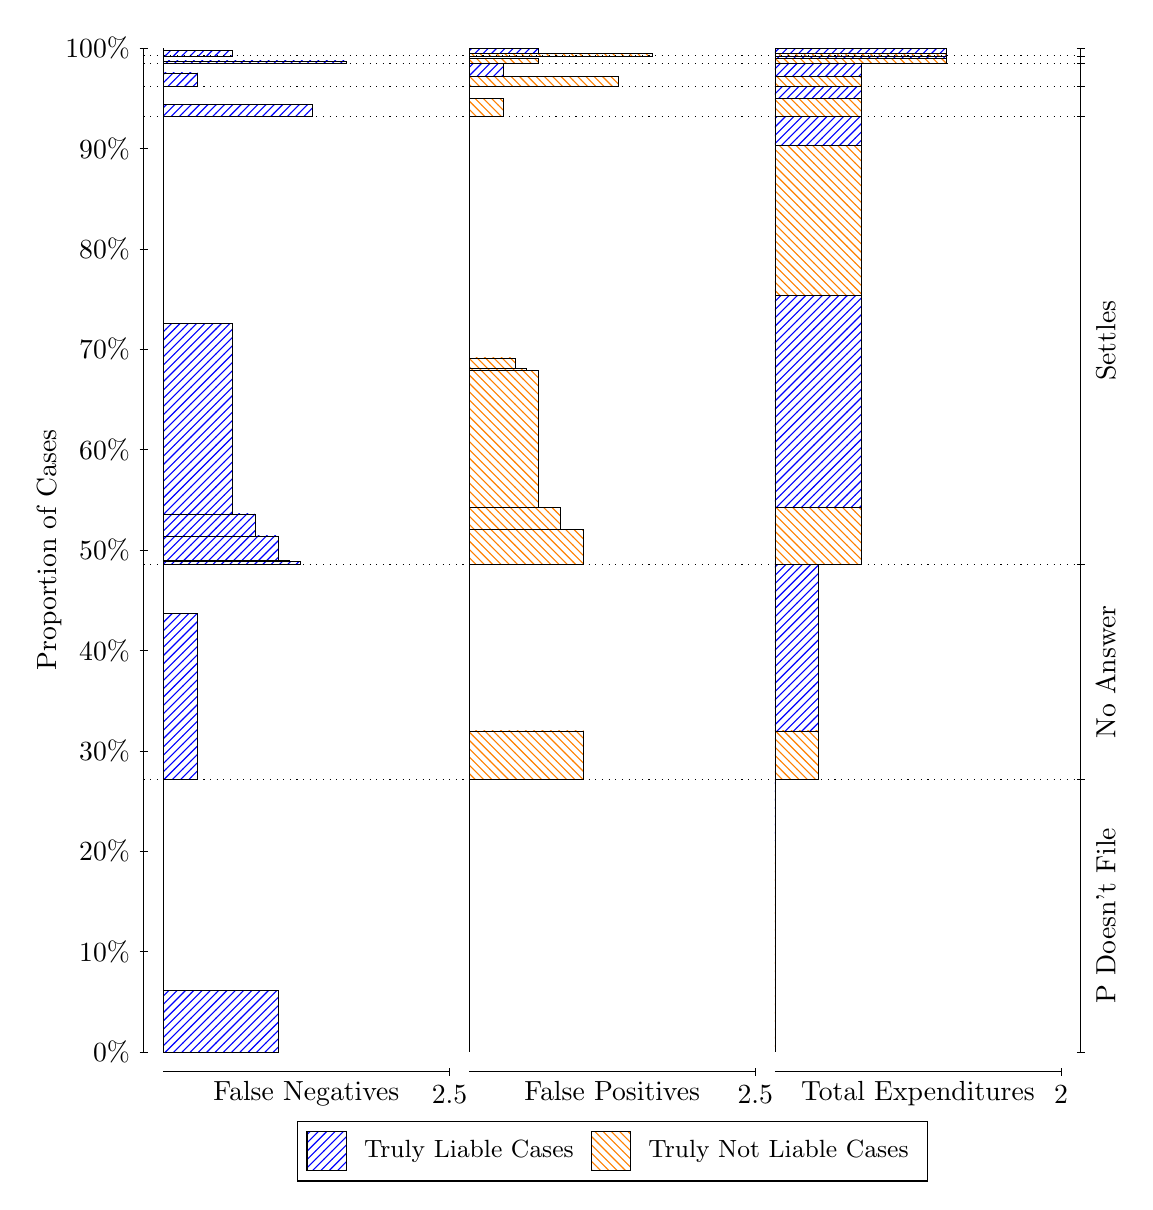
\begin{tikzpicture}
\draw[black, very thin] (1.5,1.75) -- (1.5,14.5);
\node[rotate=90, text=black, anchor=center] at (0.3, 8.125) {Proportion of Cases};
\draw[black, very thin] (1.45,1.75) -- (1.55,1.75);
\node[text=black, anchor=east] at (1.45, 1.75) {0\%};
\draw[black, very thin] (1.45,3.025) -- (1.55,3.025);
\node[text=black, anchor=east] at (1.45, 3.025) {10\%};
\draw[black, very thin] (1.45,4.3) -- (1.55,4.3);
\node[text=black, anchor=east] at (1.45, 4.3) {20\%};
\draw[black, very thin] (1.45,5.575) -- (1.55,5.575);
\node[text=black, anchor=east] at (1.45, 5.575) {30\%};
\draw[black, very thin] (1.45,6.85) -- (1.55,6.85);
\node[text=black, anchor=east] at (1.45, 6.85) {40\%};
\draw[black, very thin] (1.45,8.125) -- (1.55,8.125);
\node[text=black, anchor=east] at (1.45, 8.125) {50\%};
\draw[black, very thin] (1.45,9.4) -- (1.55,9.4);
\node[text=black, anchor=east] at (1.45, 9.4) {60\%};
\draw[black, very thin] (1.45,10.675) -- (1.55,10.675);
\node[text=black, anchor=east] at (1.45, 10.675) {70\%};
\draw[black, very thin] (1.45,11.95) -- (1.55,11.95);
\node[text=black, anchor=east] at (1.45, 11.95) {80\%};
\draw[black, very thin] (1.45,13.225) -- (1.55,13.225);
\node[text=black, anchor=east] at (1.45, 13.225) {90\%};
\draw[black, very thin] (1.45,14.5) -- (1.55,14.5);
\node[text=black, anchor=east] at (1.45, 14.5) {100\%};

\draw[black, very thin] (13.4,1.75) -- (13.4,14.5);
\draw[black, very thin] (13.35,1.75) -- (13.45,1.75);
\node[anchor=west] at (13.35, 1.75) {};
\draw[black, very thin] (13.35,5.2117) -- (13.45,5.2117);
\node[anchor=west] at (13.35, 5.2117) {};
\draw[black, very thin] (13.35,7.94) -- (13.45,7.94);
\node[anchor=west] at (13.35, 7.94) {};
\draw[black, very thin] (13.35,13.629) -- (13.45,13.629);
\node[anchor=west] at (13.35, 13.629) {};
\draw[black, very thin] (13.35,14.017) -- (13.45,14.017);
\node[anchor=west] at (13.35, 14.017) {};
\draw[black, very thin] (13.35,14.308) -- (13.45,14.308);
\node[anchor=west] at (13.35, 14.308) {};
\draw[black, very thin] (13.35,14.401) -- (13.45,14.401);
\node[anchor=west] at (13.35, 14.401) {};
\draw[black, very thin] (13.35,14.5) -- (13.45,14.5);
\node[anchor=west] at (13.35, 14.5) {};

\draw[black, very thin, pattern color=blue, pattern=north east lines] (1.75,1.75) rectangle (3.2033,2.5302);
\draw[black, very thin, pattern color=orange, pattern=north west lines] (1.75,2.5302) rectangle (1.75,5.2117);
\draw[black, very thin, pattern color=blue, pattern=north east lines] (1.75,5.2117) rectangle (2.186,7.3234);
\draw[black, very thin, pattern color=orange, pattern=north west lines] (1.75,7.3234) rectangle (1.75,7.94);
\draw[black, very thin, pattern color=blue, pattern=north east lines] (1.75,7.94) rectangle (3.494,7.9819);
\draw[black, very thin, pattern color=blue, pattern=north east lines] (1.75,7.9819) rectangle (3.3487,7.9882);
\draw[black, very thin, pattern color=blue, pattern=north east lines] (1.75,7.9882) rectangle (3.2033,8.3054);
\draw[black, very thin, pattern color=blue, pattern=north east lines] (1.75,8.3054) rectangle (2.9127,8.5836);
\draw[black, very thin, pattern color=blue, pattern=north east lines] (1.75,8.5836) rectangle (2.622,11.004);
\draw[black, very thin, pattern color=orange, pattern=north west lines] (1.75,11.004) rectangle (1.75,13.629);
\draw[black, very thin, pattern color=blue, pattern=north east lines] (1.75,13.629) rectangle (3.6393,13.783);
\draw[black, very thin, pattern color=orange, pattern=north west lines] (1.75,13.783) rectangle (1.75,14.017);
\draw[black, very thin, pattern color=blue, pattern=north east lines] (1.75,14.017) rectangle (2.186,14.183);
\draw[black, very thin, pattern color=orange, pattern=north west lines] (1.75,14.183) rectangle (1.75,14.308);
\draw[black, very thin, pattern color=blue, pattern=north east lines] (1.75,14.308) rectangle (4.0753,14.338);
\draw[black, very thin, pattern color=orange, pattern=north west lines] (1.75,14.338) rectangle (1.75,14.401);
\draw[black, very thin, pattern color=blue, pattern=north east lines] (1.75,14.401) rectangle (2.622,14.47);
\draw[black, very thin, pattern color=orange, pattern=north west lines] (1.75,14.47) rectangle (1.75,14.5);
\draw[black, very thin, pattern color=orange, pattern=north west lines] (5.6333,1.75) rectangle (5.6333,4.4314);
\draw[black, very thin, pattern color=blue, pattern=north east lines] (5.6333,4.4314) rectangle (5.6333,5.2117);
\draw[black, very thin, pattern color=orange, pattern=north west lines] (5.6333,5.2117) rectangle (7.0867,5.8282);
\draw[black, very thin, pattern color=blue, pattern=north east lines] (5.6333,5.8282) rectangle (5.6333,7.94);
\draw[black, very thin, pattern color=orange, pattern=north west lines] (5.6333,7.94) rectangle (7.0867,8.3863);
\draw[black, very thin, pattern color=orange, pattern=north west lines] (5.6333,8.3863) rectangle (6.796,8.6644);
\draw[black, very thin, pattern color=orange, pattern=north west lines] (5.6333,8.6644) rectangle (6.5053,10.411);
\draw[black, very thin, pattern color=orange, pattern=north west lines] (5.6333,10.411) rectangle (6.36,10.43);
\draw[black, very thin, pattern color=orange, pattern=north west lines] (5.6333,10.43) rectangle (6.2147,10.565);
\draw[black, very thin, pattern color=blue, pattern=north east lines] (5.6333,10.565) rectangle (5.6333,13.629);
\draw[black, very thin, pattern color=orange, pattern=north west lines] (5.6333,13.629) rectangle (6.0693,13.863);
\draw[black, very thin, pattern color=blue, pattern=north east lines] (5.6333,13.863) rectangle (5.6333,14.017);
\draw[black, very thin, pattern color=orange, pattern=north west lines] (5.6333,14.017) rectangle (7.5227,14.142);
\draw[black, very thin, pattern color=blue, pattern=north east lines] (5.6333,14.142) rectangle (6.0693,14.308);
\draw[black, very thin, pattern color=orange, pattern=north west lines] (5.6333,14.308) rectangle (6.5053,14.372);
\draw[black, very thin, pattern color=blue, pattern=north east lines] (5.6333,14.372) rectangle (5.6333,14.401);
\draw[black, very thin, pattern color=orange, pattern=north west lines] (5.6333,14.401) rectangle (7.9587,14.431);
\draw[black, very thin, pattern color=blue, pattern=north east lines] (5.6333,14.431) rectangle (6.5053,14.5);
\draw[black, very thin, pattern color=orange, pattern=north west lines] (9.5167,1.75) rectangle (9.5167,4.4314);
\draw[black, very thin, pattern color=blue, pattern=north east lines] (9.5167,4.4314) rectangle (9.5167,5.2117);
\draw[black, very thin, pattern color=orange, pattern=north west lines] (9.5167,5.2117) rectangle (10.062,5.8282);
\draw[black, very thin, pattern color=blue, pattern=north east lines] (9.5167,5.8282) rectangle (10.062,7.94);
\draw[black, very thin, pattern color=orange, pattern=north west lines] (9.5167,7.94) rectangle (10.607,8.6644);
\draw[black, very thin, pattern color=blue, pattern=north east lines] (9.5167,8.6644) rectangle (10.607,11.363);
\draw[black, very thin, pattern color=orange, pattern=north west lines] (9.5167,11.363) rectangle (10.607,13.263);
\draw[black, very thin, pattern color=blue, pattern=north east lines] (9.5167,13.263) rectangle (10.607,13.629);
\draw[black, very thin, pattern color=orange, pattern=north west lines] (9.5167,13.629) rectangle (10.607,13.863);
\draw[black, very thin, pattern color=blue, pattern=north east lines] (9.5167,13.863) rectangle (10.607,14.017);
\draw[black, very thin, pattern color=orange, pattern=north west lines] (9.5167,14.017) rectangle (10.607,14.142);
\draw[black, very thin, pattern color=blue, pattern=north east lines] (9.5167,14.142) rectangle (10.607,14.308);
\draw[black, very thin, pattern color=orange, pattern=north west lines] (9.5167,14.308) rectangle (11.697,14.372);
\draw[black, very thin, pattern color=blue, pattern=north east lines] (9.5167,14.372) rectangle (11.697,14.401);
\draw[black, very thin, pattern color=orange, pattern=north west lines] (9.5167,14.401) rectangle (11.697,14.431);
\draw[black, very thin, pattern color=blue, pattern=north east lines] (9.5167,14.431) rectangle (11.697,14.5);
\draw[black, dotted] (1.5,5.2117) -- (13.4,5.2117);
\draw[black, dotted] (1.5,7.94) -- (13.4,7.94);
\draw[black, dotted] (1.5,13.629) -- (13.4,13.629);
\draw[black, dotted] (1.5,14.017) -- (13.4,14.017);
\draw[black, dotted] (1.5,14.308) -- (13.4,14.308);
\draw[black, dotted] (1.5,14.401) -- (13.4,14.401);
\draw[black, very thin] (1.75,1.5) -- (5.3833,1.5);
\node[text=black, anchor=north] at (3.5667, 1.5) {False Negatives};
\draw[black, very thin] (5.3833,1.45) -- (5.3833,1.55);
\node[text=black, anchor=north] at (5.3833, 1.45) {2.5};

\draw[black, very thin] (5.6333,1.5) -- (9.2667,1.5);
\node[text=black, anchor=north] at (7.45, 1.5) {False Positives};
\draw[black, very thin] (9.2667,1.45) -- (9.2667,1.55);
\node[text=black, anchor=north] at (9.2667, 1.45) {2.5};

\draw[black, very thin] (9.5167,1.5) -- (13.15,1.5);
\node[text=black, anchor=north] at (11.333, 1.5) {Total Expenditures};
\draw[black, very thin] (13.15,1.45) -- (13.15,1.55);
\node[text=black, anchor=north] at (13.15, 1.45) {2};

\node[text=black, centered, rotate=90] at (13.72, 3.4808) {P Doesn't File};
\node[text=black, centered, rotate=90] at (13.72, 6.5758) {No Answer};
\node[text=black, centered, rotate=90] at (13.72, 10.784) {Settles};





\draw (7.449999999999999,1.5) node[draw=none] (baseCoordinate) {};
\begin{scope}[align=center]
        \matrix[scale=0.5, draw=black, below=0.5cm of baseCoordinate, nodes={draw}, column sep=0.1cm]{
            \node[rectangle, draw, minimum width=0.5cm, minimum height=0.5cm, pattern color=blue, pattern=north east lines] {}; &
            \node[draw=none, font=\small, text=black] (B) {Truly Liable Cases}; &
            \node[rectangle, draw, minimum width=0.5cm, minimum height=0.5cm, pattern color=orange, pattern=north west lines] {}; &
            \node[draw=none, font=\small, text=black] (B) {Truly Not Liable Cases}; \\
            };
\end{scope}

\end{tikzpicture}
\end{document}